\documentclass[10pt,aspectratio=169]{beamer}
\usepackage{amsmath}
\usepackage{subfigure}
\usepackage[style=authortitle]{biblatex}


\usetheme{Madrid}
% \pgfdeclareimage[width=\paperwidth,height=\paperheight]{bg}{ecnu_background}
% \setbeamertemplate{background}{\pgfuseimage{bg}}
\setbeamertemplate{frametitle continuation}[from second]
\useinnertheme{rectangles}
\setbeamertemplate{theorems}[numbered] 
\usecolortheme[RGB={182,11,45}]{structure}
\usefonttheme{professionalfonts}
\logo{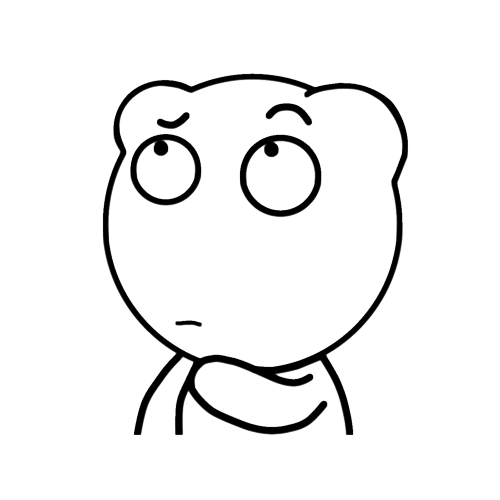
\includegraphics[width=0.12\textwidth]{logo.png}}

%%%%%%%%%%%%%%%%%%%%%%%%%%%%%%%%%%%%%%%%%%%%%%%%%%%%%%%%%%%%%%%%%%%%%%%%%%%%%%%%
\title{Introduction to Graph Neural Networks}
\subtitle{Vanilla Graph Neural Networks}
\author{Cai Shengliang}
\institute{Multi-Agent Artificial Intelligence Laboratory}
\date{November 4, 2020}
\addbibresource{main.bib}

\begin{document}
\begin{frame}
    \titlepage
\end{frame}

\begin{frame}{Outline}
    \tableofcontents
\end{frame}

\section{Introduction}
\begin{frame}{Introduction}
    \begin{itemize}[<+->]
        \item The concept of GNN was first proposed in \citeauthor{Scarselli2009} [\citeyear{Scarselli2009}], which aims to extend existing neural networks for processing graph-structured data.\footcite{liu2020introduction}
        \item A function $\tau$ that maps a graph $G$ and one of its nodes $n$  to a vector of reals: $\tau(\boldsymbol{G}, n) \in \mathbb{R} ^ m$
        \item \emph{graph-focused} and \emph{node-focused} \footcite{Scarselli2009}
    \end{itemize}
\end{frame}

\begin{frame}{Introduction}{Graph-focused}
    In \emph{graph-focused} applications, the function $\tau$ is independent of the node and implements a classifier or a regressor on a graph structured data set.

    \begin{figure}
        \centering
        \subfigure[] {
            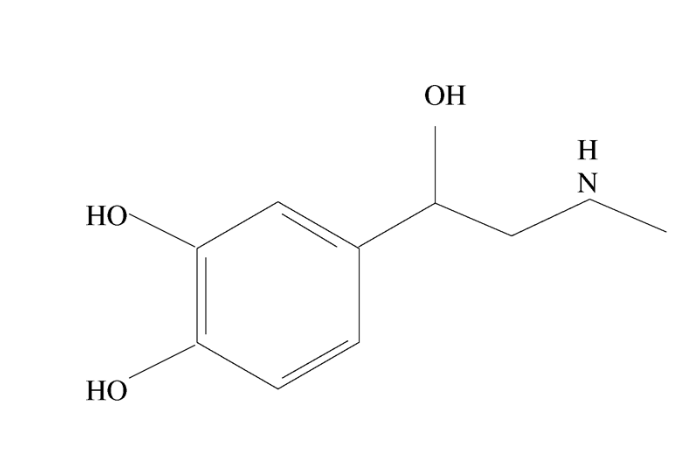
\includegraphics[width=.3\textwidth]{pic/chemical.png}
        }
        \subfigure[]{
            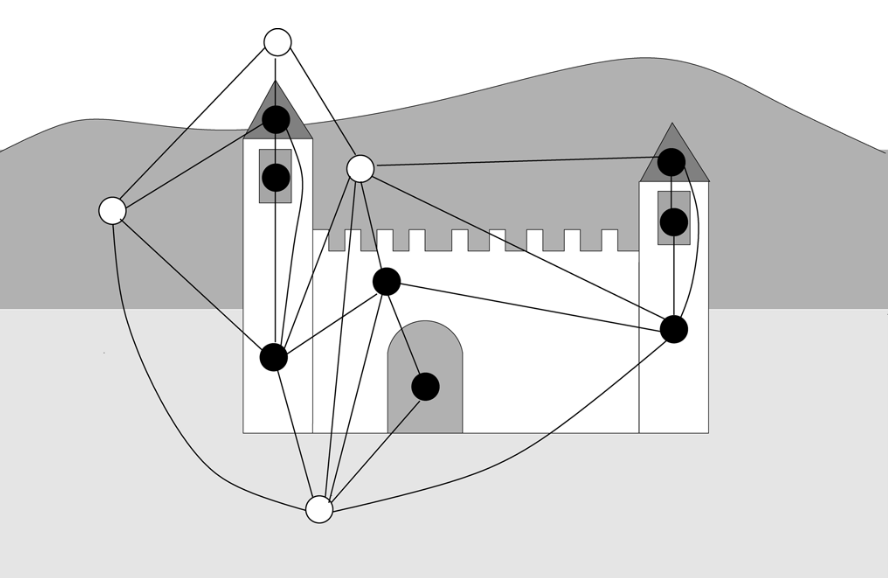
\includegraphics[width=.3\textwidth]{pic/image.png}
        }
    \end{figure}
\end{frame}

\begin{frame}{Introduction}{Node-focused}
    In \emph{node-focused} applications, $\tau$ depends on the node, so that the classification (or the regression) depends on the properties of each node.

    \begin{figure}
        \centering
        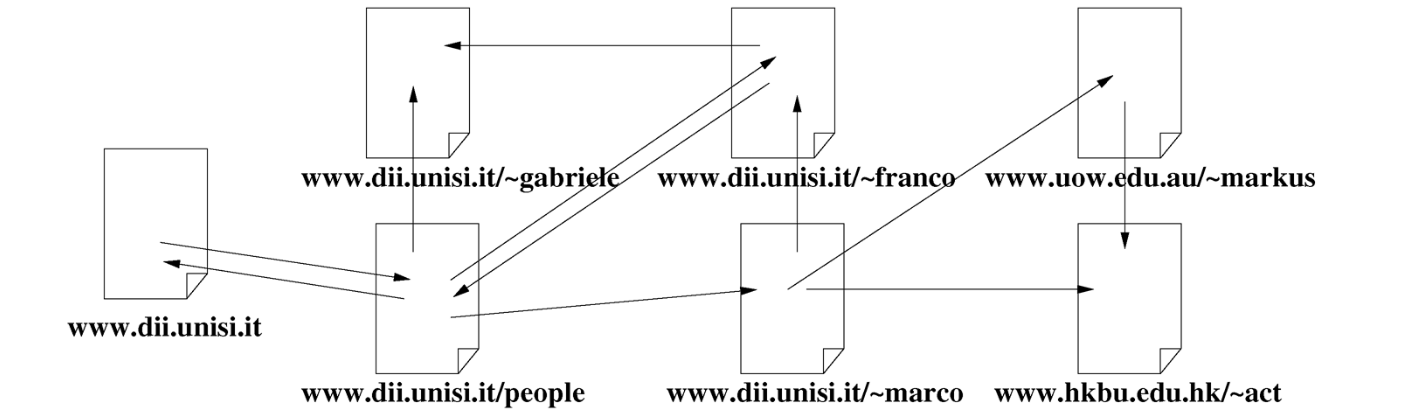
\includegraphics[width=.8\textwidth]{pic/website.png}
    \end{figure}
\end{frame}

\begin{frame}{Introduction}
    \begin{itemize}
        \item Based on an information diffusion mechanism.
        \item The units update their states and exchange information until they reach a stable equilibrium.
        \item The output of a GNN is then computed locally at each node on the base of the unit state.
    \end{itemize}
\end{frame}

\section{The graph neural network model}
\begin{frame}[allowframebreaks]{The graph neural network model}

    \begin{itemize}
        \item A graph $\boldsymbol{G}$ is a pair $(\boldsymbol{N}, \boldsymbol{E})$.
        \item $\text{ne}[x]$ --- the neighbors of $n$.
        \item $\text{co}[x]$ --- the set of arcs having $n$ as a vertex.
        \item $\boldsymbol{l}_n \in \mathbb{R} ^ {\boldsymbol{l}_{\boldsymbol{N}}}$, $\boldsymbol{l}_{(n_1, n_2)} \in \mathbb{R} ^ {\boldsymbol{l}_{\boldsymbol{E}}}$ --- labels.
    \end{itemize}

    \framebreak
    \begin{itemize}
        \item The considered graphs may be either \emph{positional} or \emph{nonpositional}.
        \item For each node $n$ in a positional graph, there exists an injective function
              $$\boldsymbol{v}_n : \text{ne}[n] \rightarrow \{1, \ldots, |\boldsymbol{N}|\}$$
        \item The domain considered in this paper is the set $\mathcal{D}$ of pairs of a graph and a node, i.e, $\mathcal{D} = \mathcal{G} \times \mathcal{N}$.
              We assume a supervised learning framework with the learning set
              where:
              $$
                  \mathcal{L}=\left\{\left(\boldsymbol{G}_{i}, n_{i, j}, \boldsymbol{t}_{i, j}\right) \mid, \boldsymbol{G}_{i}=\left(\boldsymbol{N}_{i}, \boldsymbol{E}_{i}\right) \in \mathcal{G}
                  n_{i, j} \in \boldsymbol{N}_{i} ; \boldsymbol{t}_{i, j} \in \mathbb{R}^{m}, 1 \leq i \leq p, 1 \leq j \leq q_{i}\right\}
              $$
    \end{itemize}

    \begin{figure}
        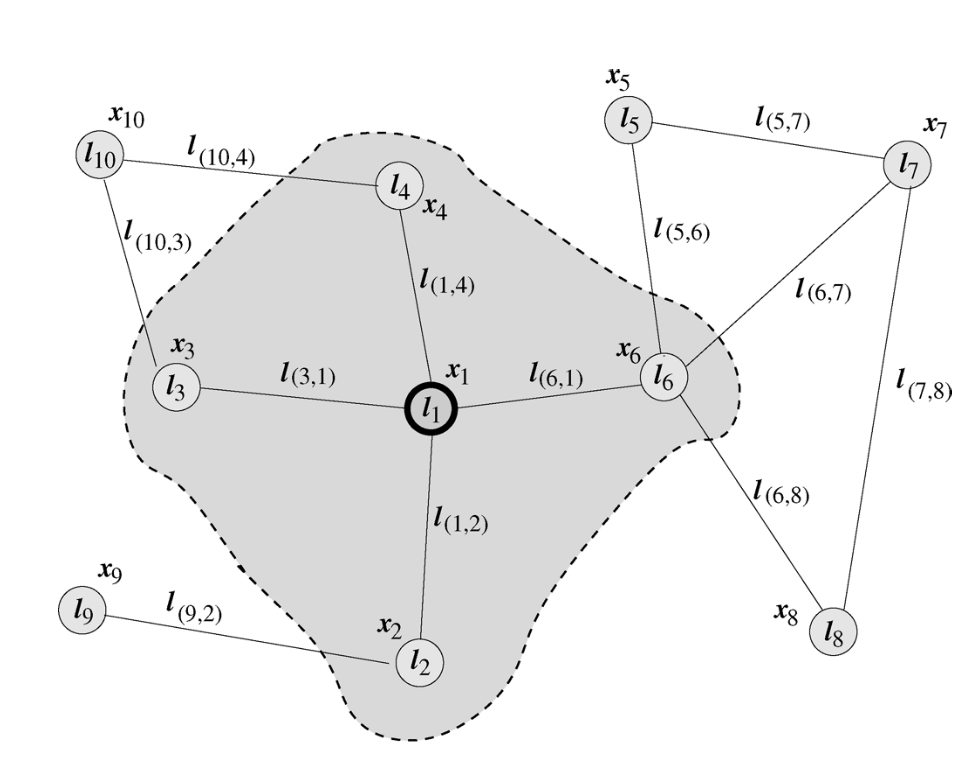
\includegraphics[width=.34\textwidth]{pic/graph.png}
        $$\boldsymbol{x}_{1}=f_{\boldsymbol{w}}(\boldsymbol{l}_{1}, \underbrace{\boldsymbol{l}_{(1,2)}, \boldsymbol{l}_{(3,1)}, \boldsymbol{l}_{(1,4)}, \boldsymbol{l}_{(6,1)}}_{\boldsymbol{l}_{\text{co}[1]}}, \underbrace{\boldsymbol{x}_{2}, \boldsymbol{x}_{3}, \boldsymbol{x}_{4}, \boldsymbol{x}_{6}}_{\boldsymbol{x}_{\text{ne}[1]}}, \underbrace{\boldsymbol{l}_{2}, \boldsymbol{l}_{3}, \boldsymbol{l}_{4}, \boldsymbol{l}_{6}}_{\boldsymbol{l}_{\text{ne}[n]}})$$
        \caption{Graph and the neighborhood of a node.}
    \end{figure}

\end{frame}

\subsection{The model}
\begin{frame}[allowframebreaks]{The model}

    \begin{itemize}
        \item $f_{\boldsymbol{w}}$: \emph{local transition function} expresses the dependence of a node $n$ on its neighborhood.
        \item $g_{\boldsymbol{w}}$: \emph{local output function} describes how the output is produced.
        \item $\boldsymbol{x}_n$ and $\boldsymbol{o}_{n}$ are defined as follows:
              \begin{equation}
                  \label{equ1}
                  \begin{aligned}
                      \boldsymbol{x}_{n} & =f_{\boldsymbol{w}}\left(\boldsymbol{l}_{n}, \boldsymbol{l}_{\mathrm{co}[n]}, \boldsymbol{x}_{\mathrm{ne}[n]}, \boldsymbol{l}_{\mathrm{ne}[n]}\right) \\
                      \boldsymbol{o}_{n} & =g_{\boldsymbol{w}}\left(\boldsymbol{x}_{n}, \boldsymbol{l}_{n}\right)
                  \end{aligned}
              \end{equation}
    \end{itemize}

    \framebreak

    \begin{itemize}
        \item It can be rewritten in a compact form as
              \begin{equation}
                  \label{equ2}
                  \begin{aligned}
                      \boldsymbol{x} & =F_{\boldsymbol{w}}(\boldsymbol{x}, \boldsymbol{l})                             \\
                      \boldsymbol{o} & =G_{\boldsymbol{w}}\left(\boldsymbol{x}, \boldsymbol{l}_{\boldsymbol{N}}\right)
                  \end{aligned}
              \end{equation}
        \item For nonpositional graphs, it is useful to replace function $f_{\boldsymbol{w}}$
              of (\ref{equ1}) with
              \begin{equation}
                  \label{equ3}
                  \boldsymbol{x}_{n}=\sum_{u \in \operatorname{ne[} n]} h_{\boldsymbol{w}}\left(\boldsymbol{l}_{n}, \boldsymbol{l}_{(n, u)}, \boldsymbol{x}_{u}, \boldsymbol{l}_{u}\right), \quad n \in \boldsymbol{N}
              \end{equation}
    \end{itemize}

    \framebreak

    In order to implement the GNN model, the following items must be provided:

    \begin{enumerate}
        \item a method to solve (\ref{equ1});
        \item a learning algorithm to adapt $f_{\boldsymbol{w}}$ and $g_{\boldsymbol{w}}$ using examples from the training data set;
        \item an implementation of $f_{\boldsymbol{w}}$ and $g_{\boldsymbol{w}}$.
    \end{enumerate}

\end{frame}

\subsection{Computation of the State}
\begin{frame}[allowframebreaks]{Computation of the State}

    According to Banach’s fixed point theorem\footcite{khamsi2011introduction}, GNN uses the follpwing classic iterative scheme to compute the state

    \begin{equation}
        \boldsymbol{x}(t + 1) = F_{\boldsymbol{w}} (\boldsymbol{x}(t), \boldsymbol{l})
    \end{equation}

    In fact, it implements \emph{the Jacobi iterative method} for solving nonlinear equations\footcites{powell1964efficient}.

    Thus, the outputs and the states can be computed by iterating
    \begin{equation}
        \label{equ5}
        \begin{aligned}
            \boldsymbol{x}_{n}(t+1) & =f_{\boldsymbol{w}}\left(\boldsymbol{l}_{n}, \boldsymbol{l}_{\mathrm{co}[n]}, \boldsymbol{x}_{\mathrm{ne}[n]}(t), \boldsymbol{l}_{\mathrm{ne}[n]}\right) \\
            \boldsymbol{o}_{n}(t)   & =g_{\boldsymbol{w}}\left(\boldsymbol{x}_{n}(t), \boldsymbol{l}_{n}\right), \quad n \in \boldsymbol{N}
        \end{aligned}
    \end{equation}
\end{frame}

\begin{frame}[allowframebreaks]
    \begin{figure}
        \centering
        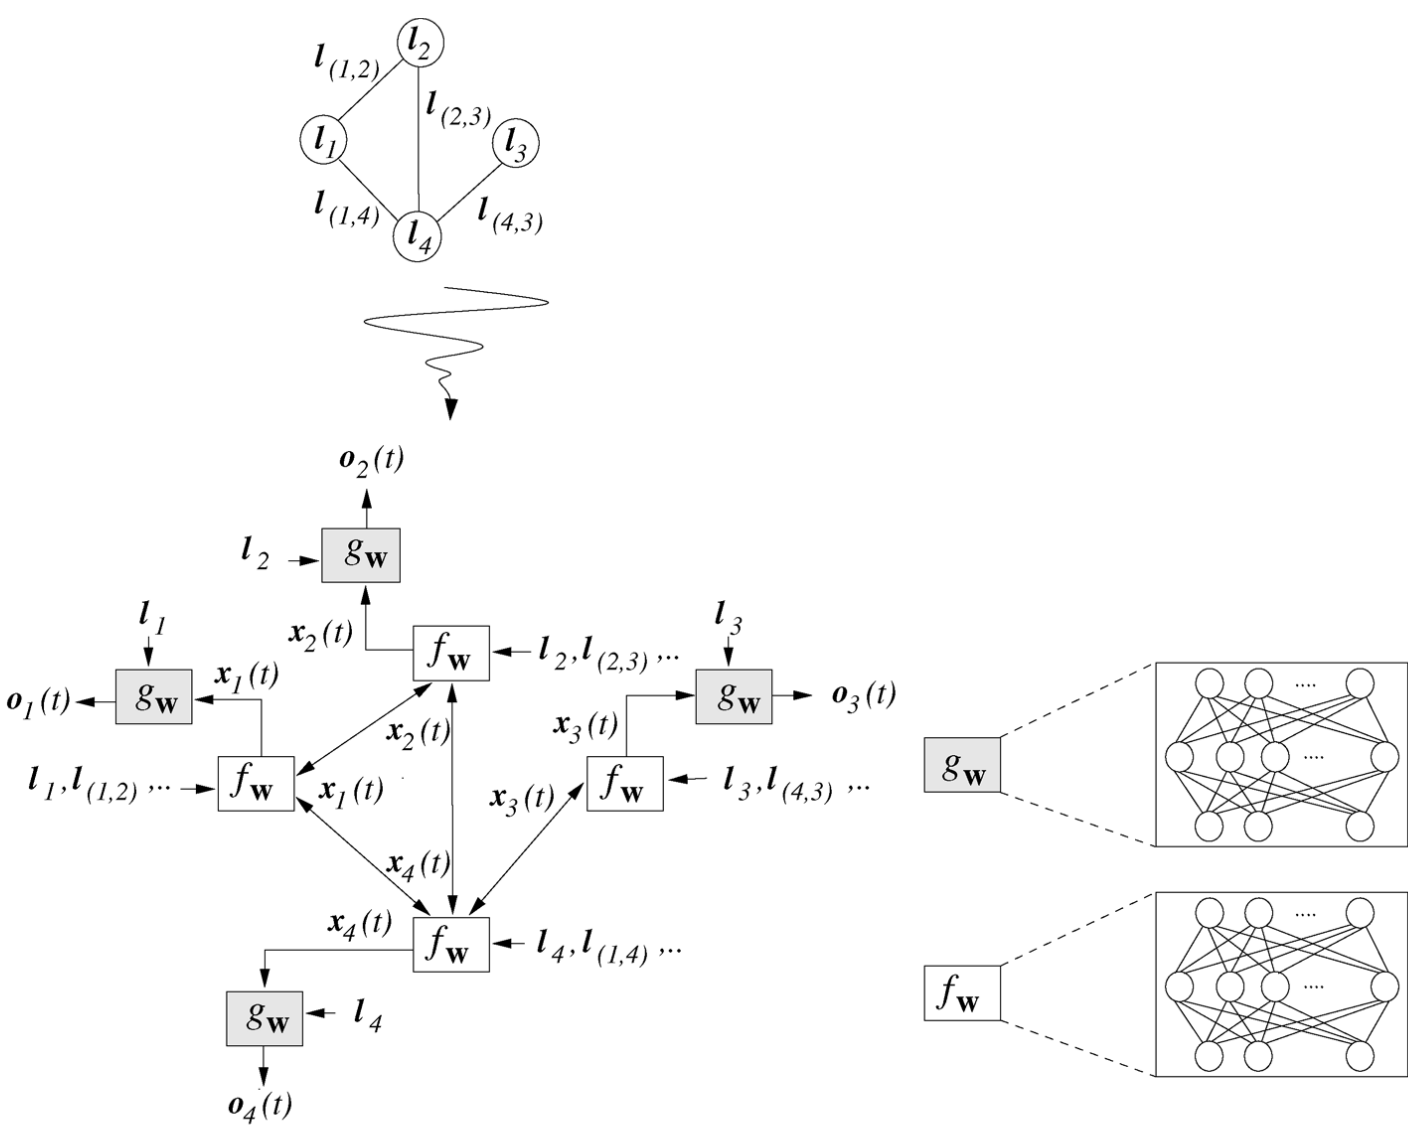
\includegraphics[width=.65\textwidth]{pic/network1.png}
    \end{figure}

    \begin{figure}
        \centering
        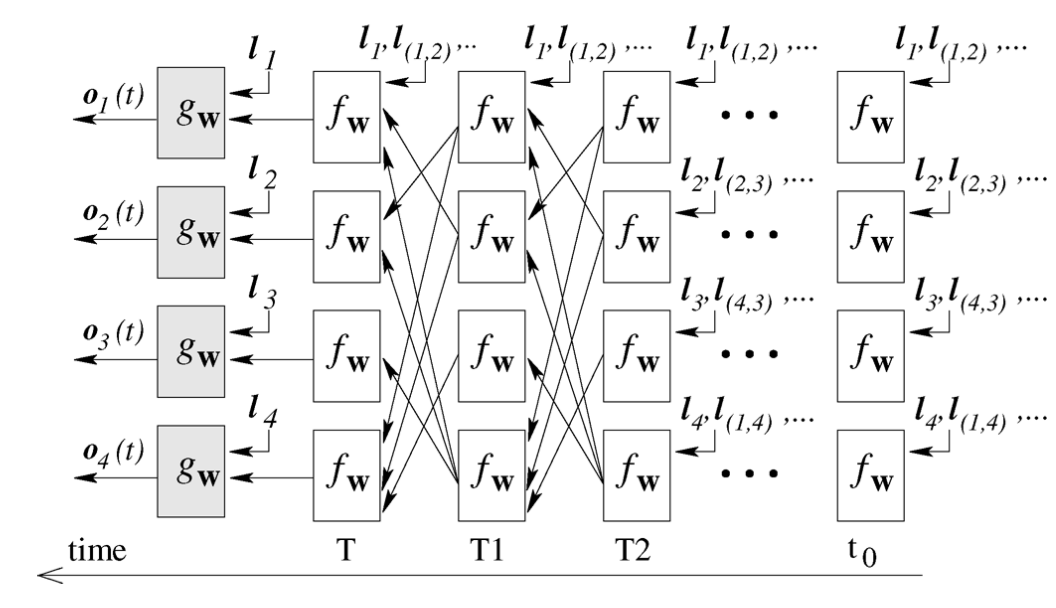
\includegraphics[width=.65\textwidth]{pic/network2.png}
    \end{figure}

\end{frame}

\subsection{The Learning Algorithm}
\begin{frame}[allowframebreaks]{The Learning Algorithm}
    \begin{itemize}
        \item Learning in GNNs consists of estimating the parameter $\boldsymbol{w}$ such that $\varphi_{\boldsymbol{w}}$ approximates the data in the learning data set
              $$
                  \mathcal{L}=\left\{\left(\boldsymbol{G}_{i}, n_{i, j}, \boldsymbol{t}_{i, j}\right) \mid, \boldsymbol{G}_{i}=\left(\boldsymbol{N}_{i}, \boldsymbol{E}_{i}\right) \in \mathcal{G}
                  n_{i, j} \in \boldsymbol{N}_{i} ; \boldsymbol{t}_{i, j} \in \mathbb{R}^{m}, 1 \leq i \leq p, 1 \leq j \leq q_{i}\right\}
              $$
        \item The learning task can be posed as the minimization of a quadratic cost function
              \begin{equation}
                  e_{\boldsymbol{w}}=\sum_{i=1}^{p} \sum_{j=1}^{q_{i}}\left(\boldsymbol{t}_{i, j}-\varphi_{\boldsymbol{w}}\left(\boldsymbol{G}_{i}, n_{i, j}\right)\right)^{2}
              \end{equation}
    \end{itemize}

    \framebreak

    \begin{enumerate}[a]
        \item The state $\boldsymbol{x}_n(t)$ are iteratively updated by (\ref{equ5}) until at time $T$ they approach the fixed point solution of (\ref{equ2}): $\boldsymbol{x}(T) \approx \boldsymbol{x}$;
        \item The gradient $\partial e_{\boldsymbol{w}}(T) / \partial \boldsymbol{w}$ is computed;
        \item The weight $\boldsymbol{w}$ are updated according to the gradient computed in step b).
    \end{enumerate}

    \framebreak

    The following two theorems show that such an intuitive
    approach has a formal justification.

    \begin{theorem}{Differentiability}
        Let $F_{\boldsymbol{w}}$ and $G_{\boldsymbol{w}}$ be the global transition and the global output functions of a GNN, respectively. If $F_{\boldsymbol{w}}(\boldsymbol{x}, \boldsymbol{l})$ and $G_{\boldsymbol{w}}\left(\boldsymbol{x}, \boldsymbol{l}_{\boldsymbol{N}}\right)$ are continuously differentiable w.r.t. $x$ and $w,$ then $\varphi_{w}$ is continuously differentiable w.r.t. $\boldsymbol{w}$.
    \end{theorem}

    \begin{tiny}
        The proof is left as an exercise.
    \end{tiny}

    \begin{theorem}{Backpropagation}
        Let $F_{\boldsymbol{w}}$ and $G_{\boldsymbol{w}}$ be the transition and the output functions of a GNN, respectively, and assume that $F_{\boldsymbol{w}}(\boldsymbol{x}, \boldsymbol{l})$ and $G_{\boldsymbol{w}}\left(\boldsymbol{x}, \boldsymbol{l}_{\boldsymbol{N}}\right)$ are continuously differentiable w.r.t. $x$ and $w$. Let $\boldsymbol{z}(t)$ be defined by
        \begin{equation}
            \boldsymbol{z}(t)=\boldsymbol{z}(t+1) \cdot \frac{\partial F_{\boldsymbol{w}}}{\partial \boldsymbol{x}}(\boldsymbol{x}, \boldsymbol{l})+\frac{\partial e_{\boldsymbol{w}}}{\partial \boldsymbol{o}} \cdot \frac{\partial G_{\boldsymbol{w}}}{\partial \boldsymbol{x}}\left(\boldsymbol{x}, \boldsymbol{l}_{\boldsymbol{N}}\right)
        \end{equation}
        Then, the sequence $\boldsymbol{z}(T), \boldsymbol{z}(T-1), \ldots$ converges to a vector $\boldsymbol{z}=\lim _{t \rightarrow-\infty} \boldsymbol{z}(t)$ and the convergence is exponential and independent of the initial state $\boldsymbol{z}(T) .$ Moreover
        \begin{equation}
            \frac{\partial e_{\boldsymbol{w}}}{\partial \boldsymbol{w}}=\frac{\partial e_{\boldsymbol{w}}}{\partial \boldsymbol{o}} \cdot \frac{\partial G_{\boldsymbol{w}}}{\partial \boldsymbol{w}}\left(\boldsymbol{x}, \boldsymbol{l}_{\boldsymbol{N}}\right)+\boldsymbol{z} \cdot \frac{\partial F_{\boldsymbol{w}}}{\partial \boldsymbol{w}}(\boldsymbol{x}, \boldsymbol{l})
        \end{equation}
        holds, where $x$ is the stable state of the GNN.
    \end{theorem}


    \framebreak
    \begin{figure}
        \centering
        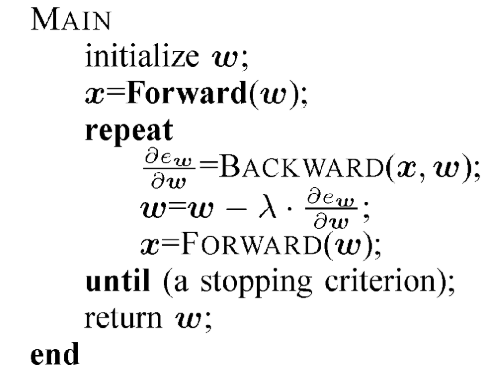
\includegraphics[width=0.3\textwidth]{pic/main.png}
        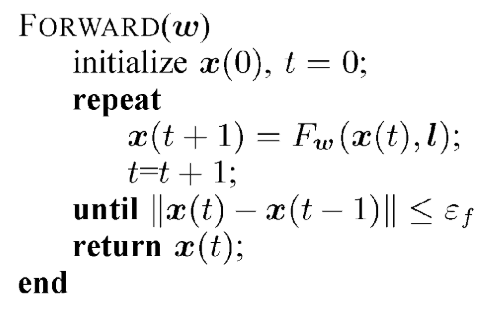
\includegraphics[width=0.3\textwidth]{pic/forward.png}
        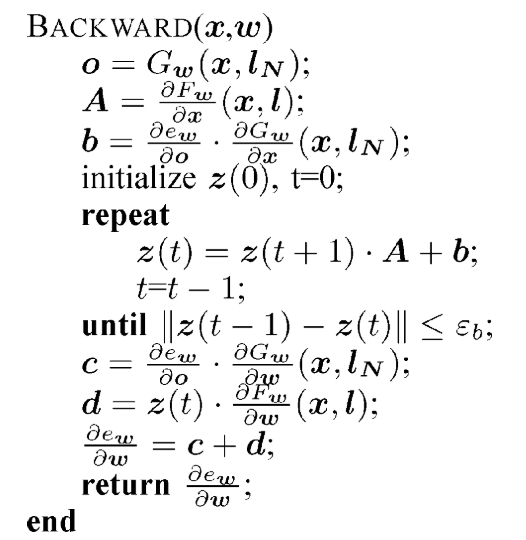
\includegraphics[width=0.3\textwidth]{pic/backward.png}
    \end{figure}

\end{frame}

\subsection{Transition and Output Function Implementations}
\begin{frame}[allowframebreaks]{Transition and Output Function Implementations}
    \begin{itemize}
        \item Linear (nonpositional) GNN

              Equation (\ref{equ3}) can naturally be implemented by
              \begin{equation}
                  h_{\boldsymbol{w}}\left(\boldsymbol{l}_{n}, \boldsymbol{l}_{(n, u)}, \boldsymbol{x}_{u}, \boldsymbol{l}_{u}\right)=\boldsymbol{A}_{n, u} \boldsymbol{x}_{u}+\boldsymbol{b}_{n}
              \end{equation}
              \begin{equation}
                  A_{n, u} =\frac{\mu}{s|\operatorname{ne}[u]|} \cdot \Xi
              \end{equation}
              \begin{equation}
                  b_{n} =\rho_{\boldsymbol{w}}\left(l_{n}\right)
              \end{equation}

              where $\mu \in(0,1)$ and $\Xi=\operatorname{resize}\left(\phi_{\boldsymbol{w}}\left(\boldsymbol{l}_{n}, \boldsymbol{l}_{(n, u)}, \boldsymbol{l}_{u}\right)\right)$ hold.

              \framebreak

        \item Nonelinear(nonpositional) GNN

              In this case, is realized by a multilayered FNN.

              \begin{equation}
                  e_{\boldsymbol{w}}=\sum_{i=1}^{p} \sum_{j=1}^{q_{i}}\left(\boldsymbol{t}_{i, j}-\varphi_{\boldsymbol{w}}\left(\boldsymbol{G}_{i}, n_{i, j}\right)\right)^{2}+\beta L\left(\left\|\frac{\partial F_{\boldsymbol{w}}}{\partial \boldsymbol{x}}\right\|\right)
              \end{equation}

              where the penalty term $L(y)$ is $(y-\mu)^{2}$ if $y>\mu$ and 0 otherwise, and the parameter $\mu \in(0,1)$ defines the desired contraction constant of $F_{\boldsymbol{w}}$.

    \end{itemize}
\end{frame}

\subsection{A Comparison With Random Walks and Recursive Neural Networks}
\begin{frame}{A Comparison With Random Walks and Recursive Neural Networks}
    \begin{itemize}
        \item Recursive neural networks\footcite{frasconi1998general} are a special case of GNNs, where:
              \begin{itemize}
                  \item the input graph is a directed acyclic graph;
                  \item the inputs of $f_{\boldsymbol{w}}$ are limited to $\boldsymbol{l}_n$ and $\boldsymbol{x}_{\text{ch}[n]}$, where is the set of children of $n$;
                  \item there is a supersource node from which all the other nodes can be reached. This node is typically used for output $\boldsymbol{o}_{sn}$(graph-focused tasks).
              \end{itemize}\pause
        \item The GNN model captures also the random walks on graphs when choosing $f_{\boldsymbol{w}}$ as a linear function.
              \begin{itemize}
                  \item In random walks on graphs, the state $\boldsymbol{x}_n$ associated with a node is a real value and is described by
                        $$
                            \boldsymbol{x}_n = \sum_{i \in \text{pa}[n]} a_{n, i}\boldsymbol{x}_i
                        $$
              \end{itemize}
    \end{itemize}


\end{frame}

\section{Limitations}
\begin{frame}{Limitations}
    \begin{itemize}
        \item It is computationally inefficient to update the hidden states of nodes iteratively to get the fixed point.
        \item Vanilla GNN uses the same parameters in the iteration.
        \item There are also some informative features on the edges which cannot be effectively modeled in the vanilla GNN.
        \item If $T$ is pretty large, it is unsuitable to use the fixed points if we focus on the representation of nodes instead of graphs.
    \end{itemize}
\end{frame}

\section*{References}
\begin{frame}{References}
    \printbibliography
\end{frame}

\begin{frame}
    \begin{center}
        \Huge{Thanks for watching!}
    \end{center}
\end{frame}


\end{document}
